%%%%%%%%%%%%%%%%%%%%%%%%%%%%%%%%%%%%%%%%%%%%%%%%%%%%%%%%%%%%%%%%%%%%%%%%%%%%%%%%
%2345678901234567890123456789012345678901234567890123456789012345678901234567890
%        1         2         3         4         5         6         7         8

\documentclass[letterpaper, 10 pt, conference]{ieeeconf}  % Comment this line out
                                                          % if you need a4paper
%\documentclass[a4paper, 10pt, conference]{ieeeconf}      % Use this line for a4
                                                          % paper

\IEEEoverridecommandlockouts                              % This command is only
                                                          % needed if you want to
                                                          % use the \thanks command
\overrideIEEEmargins
% See the \addtolength command later in the file to balance the column lengths
% on the last page of the document
\usepackage{url}
\newcommand\tab[1][1cm]{\hspace*{#1}}
%graphics
\usepackage{graphicx}
%
\usepackage{hyperref}
% Enable hyperref without colors and without bookmarks
\hypersetup{hidelinks,
  colorlinks=true,
  allcolors=black,
  pdfstartview=Fit,
  breaklinks=true}
\usepackage[capitalise,nameinlink]{cleveref}
% Enable correct jumping to figures when referencing
\usepackage[all]{hypcap}
\crefname{section}{Sect.}{Sect.}
\Crefname{section}{Section}{Sections}
\crefname{listing}{\lstlistingname}{\lstlistingname}
\Crefname{listing}{Listing}{Listings}

% Used for displaying a sample figure. If possible, figure files should
% be included in EPS format.
%
% If you use the hyperref package, please uncomment the following line
% to display URLs in blue roman font according to Springer's eBook style:
\renewcommand\UrlFont{\color{blue}\rmfamily}

% The following packages can be found on http:\\www.ctan.org
%\usepackage{graphics} % for pdf, bitmapped graphics files
%\usepackage{epsfig} % for postscript graphics files
%\usepackage{mathptmx} % assumes new font selection scheme installed
%\usepackage{times} % assumes new font selection scheme installed
%\usepackage{amsmath} % assumes amsmath package installed
%\usepackage{amssymb}  % assumes amsmath package installed

%
\title{Direct File Transfer System via WebRTC\\\textit{An Alternative to E-mail Attachments with Improved Security}}
\author{Robin Lunde, Mobile And Ubiquitous Internet\\
Keio University Shonan Fujisawa Campus\\
\\
Main advisor:\tab Keiji Takeda\tab Co-advisors:\tab Jun Murai\\
\tab[5cm] \tab \tab \tab \tab \tab[1.2cm] Osamu Nakamura
}


\begin{document}

\maketitle
\thispagestyle{empty}
\pagestyle{empty}

%
\maketitle              % typeset the header of the contribution
%Creates full width text
%[
%\section{First Section}
%All human things are subject to decay. And when fate summons, Monarchs must obey.
%]

%%%%%%%%%%%%%%%%%%%%%%%%%%%%%%%%%%%%%%%%%%%%%%%%%%%%%%%%%%%%%%%%%%%%%%%%%%%%%%%%%%%%%%%%%%%%%
\begin{abstract}
Utilizing WebRTC's P2P technology, this thesis will suggest an alternative to the way e-mail attachments currently work. In today's technical environment, there are countless new and secure ways to send files over the Internet. Yet most people still use the traditional, outdated e-mail attachment technology to share files. This thesis will propose a new system that seeks to improve overall security and usability of transferring files.

The system will be evaluated against the current e-mail system, as well as cloud and SNS based solutions. The comparison will largely be focused on security and usability. This thesis will clearly show that the current e-mail system is not sufficient when it comes security, usability, or both. It will propose a solution that raises the standard of security and confidentiality, which improves the current conditions and offers an alternative solution.

It suggests a system utilizing the web of trust model combined with WebRTC's P2P functionality. By using the web of trust model, the end-user gets more control over whom he trusts, while simultaneously avoiding the problem of having to authenticate users against a central server or service. The P2P functionality of WebRTC allows for the direct transfer of files between users, avoiding the need for servers to store the files in transit. This reduces the risk of an attacker gaining access to the file, while also optimizing transfer-speed. This system was implemented in a prototype to demonstrate the feasibility of the proposed system.
%
\end{abstract}
%
\section{Introduction}
%
SendIt's primary goal is to be an easy to use application for improving security when transferring files. It aims to reduce the risk of data theft while still being usable by people lacking technical insight. It also aims to improve the security compared to commonly used solutions. We believe there is a lack of good solutions currently available. This is illustrated by the fact that it is not uncommon for a decryption-key and cipher to be sent over the same channel when sharing encrypted files. This holds true even for security specialists! 

There is also a global trend towards higher requirements regarding data protection and handling, as demonstrated by EU's new General Data Protection Regulation \cite{law_gdpr,ar_gdpr} and Special Publication 800-171 in the US. \cite{law_sp800} There is a strong demand to minimize exposure of personal data. With this in mind, we seek to be in compliance with these trends. 

We also seek to utilize peer-to-peer technology, as it keeps in mind the original idea of the internet being a decentralized system. \cite{ar_decent} It also allows SendIt to directly transfer the file, without having to store it anywhere in transit. This reduces the attack surface, reducing the risk of leaking data.
%
\section{Related work}
%
\subsection{Existing solutions}
There exists solutions available and under development that resemble SendIt. FireFox Send \cite{url_firesend} is a service that aims to make sending files easier in an encrypted fashion. They are using a cloud service to store the file. The link expires after 24 hours or the indicated number of downloads. This is in contrast to SendIt's direct solution.

Tox is a solution that is fairly similar to SendIt. It uses DHT to create a network layer for finding connections and another DHT network layer for connection setup between nodes. This results in a decentralized, P2P network with end-to-end encryption. Unfortunately using DHT means it is harder to maintain and deploy, and that one needs to enter the DHT through certain nodes. These problems are not present in SendIt. \cite{url_tox,url_toxdoc}

There is also an existing implementation that we used as a reference for SendIt. The Serverless-WebRTC solution \cite{url_webrtc_ex} was the proof of concept that inspired SendIt.
%
\subsection{Contributions}
Many solutions to share files already exists, with a few mentioned above. Both Tox and SendIt use a direct, serverless solution, which is a rare approach. The exchange and management of identities combined with peer-to-peer transfer and trust evaluation is original to the suggested system. The combination of these technologies, constitutes my original research activities. In summary, a direct transfer system, based on non-absolute trust for the first interaction, is original to this system.
%
\section{System}
%
SendIt uses e-mail addresses as usernames in order to have unique identities. It relies on non-absolute trust for the first interaction, after which a keys are exchanged and used for authentication from then on. The reason for choosing this solution is that it allows for an easy and convenient way to start communicating with new partners. It is important that the system is kept simple, to make sure it stays user friendly.

While the first exchange is not encrypted, all subsequent communications are. This guarantees that we are communicating with the same identity as before, and that all communication is confidential and can not be changed in transit. This is done using Public-key cryptography combined with session keys. A public and private key is generated and linked to each identity. A new session key is generated for every session and used to encrypt the data being transferred. This session key is encrypted using the public key of the other node before being shared, to ensure confidentiality.

\subsection{Use and use-cases}
SendIt's primary use-case is when sharing sensitive or critical data. It can also be used if you want comparatively better privacy, simple file-sharing, et cetra, compared to regular e-mail attachments. It is also compliant with the regulations previously mentioned. In short, it is a user friendly system with focus on privacy and security.

SendIt achieves this by implementing two different ways to create a peer-to-peer connection between two nodes as shown in \Cref{fig:fig1}. The file is always transferred over a secure P2P-channel and with end-to-end encryption.
\begin{figure}
  \includegraphics[width=90mm]{ACS_comparison}
  \caption{Left: Assited Connection Setup Mode, Right: Serverless mode} \label{fig:fig1}
\end{figure}
\subsection{Technology}
There are three base technologies used in SendIt. The first is WebRTC, which is used to create peer-to-peer connection for transferring the data directly. This is done by exchanging an offer and an answer containing information on how to create the connection. The second is Electron; used to create a client application without needing any server involvement. It also makes building a desktop application using web-technology possible, as well as easy application deployment. Finally, the web of trust model is used to manage and evaluate trust in identities. This is used to minimize risk of attacks and to update and re-evaluate each identity's trustworthiness. It also allows there to be a somewhat shared consensus in the system, about which identities are trustworthy.
%
\section{Evaluation of SendIt}
%
  To understand the contribution and usability of SendIt, an analysis of existing solutions is needed. By comparing SendIt with existing solutions it is possible to get an idea of what has been improved, what stayed the same, and what still needs to be improved. In the following section SendIt will be compared to the e-mail system and a generic SNS system, and the findings will be evaluated and analyzed.

  SendIt has fewer weaknesses than the other two systems. This evaluation will not include all attack vectors, but rather focus on the weaknesses that come as a consequence of the proposed system and it's design.
%
  \subsection{Possible limitations}
    %First trust!!!
    \subsubsection{First trust}
    %
    The main limitation is the first trust. This can allow an attacker to appear as the legitimate owner of an identity, without this being the case. This is a risk that any user should be aware of, as it is a critical part of the system. Even though it is a part of the design choice, it has to be acknowledged that this is less than optimal.

    The mitigation for such attacks is split in two parts. The first is relying on the user to evaluate whether the user is legitimate. By using social cues like timing, each user should evaluate if it is likely that the other identity would initiate a transfer. One can also contact the other endpoint and confirm that it is actually them. This is, of course, \textbf{only necessary for the first connection}.

    The second is the trust model, which is an automatic part of the system. It combats this issue by sharing information and allowing users to have as much data as possible, for all identities. This allows for detection of false identities and will eventually make these identities untrusted entities in the whole system.
   
    %ACS!!!
    \subsubsection{ACS}
    %
    Another attack vector is the ACS server. If it is not trusted, it can pose a security risk, as the endpoint has to rely on the fact that the ACS server relays the data to the correct recipient. If the data sent is encrypted, it will not pose any immediate risk, but it will stop the endpoint from connecting to anyone, as the other endpoint will not get authenticated properly. If it is the first time these endpoints are connecting, however, it puts the victim at risk of being put in touch with the wrong identity.

    The ACS server can also act as a logger that keeps track of which identities are communicating with each other. While not directly an attack, it can raise privacy issues, since it allows for monitoring of traffic. It can also be argued that it can be used for reconnaissance, which allows for a targeted attack on one of the endpoints. Because of this, endpoints should only use ACS servers they trust.

  \subsection{Advantages}
    \subsubsection{Connection setup}
    While P2P transfer is direct communication between two endpoints, it needs some way to set up the connection. DHT solutions rely on connecting to specific endpoints, called bootstrapping, to enter the network. This is predictable behavior that can be exploited by attackers, and it also increases the difficulty of using the system.

    As such, the system suggested leaves it up to the end users to decide how to share the information, as it is unpredictable and allows for easier usage of the system. It removes the need for any bootstrapping or server, and does not specify any set way to share the connection information.

    \subsubsection{Direct transfer}
    %No temporary storage - direct transfer
    The biggest advantage SendIt has over the other systems, is that it transfers the file directly. None of the issues stemming from files being stored in transit applies to SendIt. These issues range from attackers hacking the server and getting access to the files, to allowing attackers to monitor data going through the server, since the data will always pass through this point. As a general rule, a resource is more secure, the fewer copies exist, since it limits the attack surface.

    %Files will be broken if given enough time
    Another point to take into consideration is that even if only encrypted data is stored on a server, if an attacker gets access to the data, it is only a question of how long it takes to break the encryption. As such, minimizing the risk of leaking any data should be considered critical. This is why direct transfer of files offer such an advantage.

    %Lower attack surface - direct transfer (TIME!)
    The attack surface which is exposed is also important to evaluate. Having a server store the files, means the attack surface is quite large, since it is always online. With SendIt's direct transfer function, the file is only available during transfer. The time difference for how long the file is available to be attacked is huge. As such, this is another advantage of direct transfer, since the attack surface is significantly reduced.

    \subsubsection{Content control}
    %All content received
    In the other two systems, one is also not able to stop unwanted content. If someone shares a file, it will be delivered to the receiver's PC, or at least their e-mail server / cloud account. This is unfortunate, since receiving malicious files may cause them to be executed at a later time, or by an unintended action. It is also possible that they may execute without the user knowingly doing so. As such, it is optimal for the user to be able to stop the transfer of unwanted files, something which SendIt supports.
    %Automated spreading
    Automatic spreading of malicious files is a big problem. Files are spread to all the victim's contacts and keeps spreading in a similar fashion. While SendIt has no direct solution to mitigate this, the fact that it does not support multicast, and that the files cannot be automatically received, naturally resolves this issue.
  %
    \subsection{False E2E encryption}
    %'E2E encryption' not real - skype!
    \begin{figure}[th]
      \centering
      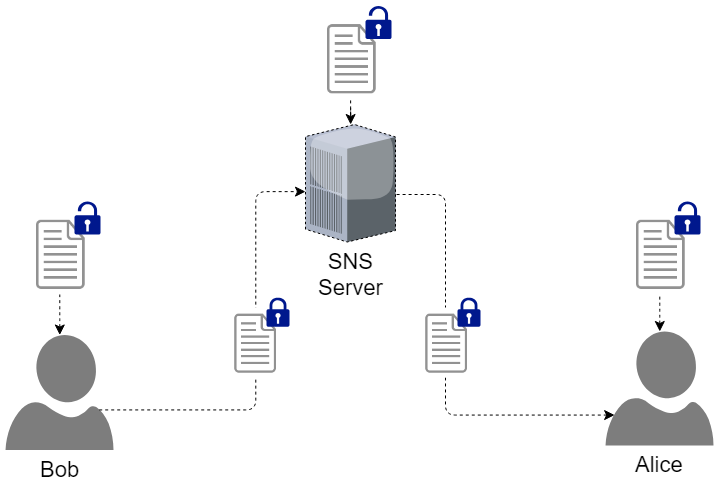
\includegraphics[width=60mm]{SNS}
      \caption[SNS: False E2E encryption]{False end-to-end encryption used in some SNS. The service has access to the keys used to encrypt the data. This allows the service to decrypt the data you send.}
      \label{fig:sns}
    \end{figure}
    As shown in \Cref{fig:sns}, false E2E encryption is sometimes utilized in cloud- and SNS-systems \cite{SkypeSecurity2018, popaSkypeProvidedBackdoor,greenwaldMicrosoftHandedNSA2013}. This is a scary thing, as a consumer of these services, because both you and your communication partner are unable to verify if the communication has true E2E encryption or not. Effectively, this is a MITM-attack by design. As such, when using these services, one should assume that the data can be decrypted and read by the service and whoever they disclose the data to. For SendIt, the public-key cryptography guarantees end-to-end encryption, since the keys are exchanged over P2P, which means no central service can tamper with the keys sent. 

\section{Conclusion}
We have proposed a new prototype and system for transferring files. SendIt is using P2P communication to avoid having to go through a server to share files. Since this makes the system vulnerable to multiple kinds of attacks, an authentication scheme based on public-key cryptography is suggested.

Since there is no central authority to vouch for any of the keys or identities used, the solution combines the above technologies with a trust-system based on the web of trust model. This is a reputation based, decentralized model which allows each user to make their own choices, while still having a shared understanding of how trustworthy each identity is. This system clearly offers some improvements to the current solutions and gives a new perspective on trust establishment. All in all, we believe that SendIt is a good alternative to the way current e-mail file attachments work, while still having room for improvement.
%
\begin{thebibliography}{99}
%1
\bibitem{law_gdpr}
Regulation (EU) 2016/679 of the European Parliament and of the Council of 27 April 2016 on the protection of natural persons with regard to the processing of personal data and on the free movement of such data, and repealing Directive 95/46/EC (General Data Protection Regulation) (Text with EEA relevance). (2016).
%2
\bibitem{ar_gdpr}
Kiesel, J.: GDPR Compliance: Summary \& Requirements You Need to Know, \url{https://linfordco.com/blog/gdpr-compliance-requirements/}, (2017).
%3
\bibitem{law_sp800}
Ross, R., Viscuso, P., Guissanie, G., Dempsey, K., Riddle, M.: Protecting controlled unclassified information in nonfederal systems and organizations. National Institute of Standards and Technology, Gaithersburg, MD (2016).
%4
\bibitem{ar_decent}
Ibanez, L.-D., Simperl, E., Gandon, F., Story, H.: Redecentralizing the Web with Distributed Ledgers. IEEE Intelligent Systems. 32, 92–95 (2017).
%5
\bibitem{url_firesend}
Firefox Test Pilot - Send, \url{https://testpilot.firefox.com/experiments/send/}. Last accessed 20 Mar 2018
%6
\bibitem{url_tox}
The Tox Project, \url{https://tox.chat/about.html}, Last accessed 15 May 2018
%7
\bibitem{url_toxdoc}
Tox protocol specification, \url{https://toktok.ltd/spec.html#introduction}, Last accessed 15 May 2018
%8
\bibitem{url_webrtc_ex}
Serverless-webRTC, \url{https://github.com/cjb/serverless-webrtc}, Last accessed 20 Mar 2018
%9
\bibitem{ar_webrtc_dc}
Jesup, R., Loreto, S. and Tuexen, M.: WebRTC data channels. draft-ietf-rtcweb-data-channel-13. txt, work in progress. (2015)
%10
\bibitem{ar_pgp}
Alfarez A.: The PGP Trust Model. EDI-Forum: the Journal of Electronic Commerce \textbf{10}(3), 27--31 (1997)
%11
\bibitem{SkypeSecurity2018}
Greenwald, G. et al. Microsoft Handed the NSA Access to Encrypted Messages.
In: The Guardian. US news (). ISSN: 0261-3077. \url{http://www.theguardian.com/world/2013/jul/11/microsoft-nsa-collaboration-user-data}, Last accessed 06 Jul 2018
%12
\bibitem{popaSkypeProvidedBackdoor}
Popa, B. Skype Provided Backdoor Access to the NSA Before Microsoft Takeover
[NYT]. URL: \url{http://news.softpedia.com/news/Skype-Provided-BackdoorAccess-to-the-NSA-Before-Microsoft-Takeover-NYT-362384.shtml}, Last accessed 06 Jul 2018
%13
\bibitem{greenwaldMicrosoftHandedNSA2013}
Is It Safe to Transfer Files via Skype?, \url{http://smallbusiness.chron.com/
safe-transfer-files-via-skype-66706.html}, Last accessed 06 Jul 2018

%
\end{thebibliography}
\end{document}